
\begin{figure}
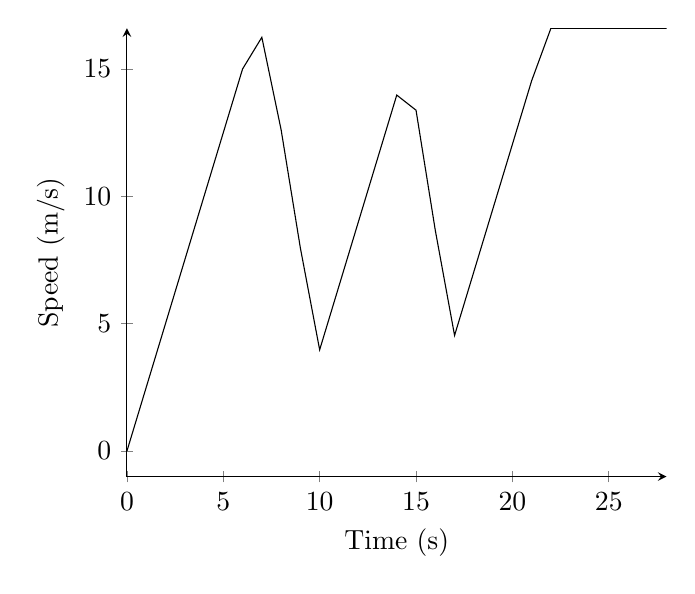
\begin{tikzpicture}
\begin{axis}[
legend style={anchor=west},
axis x line=bottom,
axis y line=left,
ymin=-1,
xlabel=Time (s),
ylabel=Speed (m/s),
]
\addplot[] coordinates {
(0, 0.0)
(1, 2.5)
(2, 5.0)
(3, 7.5)
(4, 10.0)
(5, 12.5)
(6, 15.0)
(7, 16.2437643867)
(8, 12.614908739)
(9, 7.96910600191)
(10, 3.97530202398)
(11, 6.47530202398)
(12, 8.97530202398)
(13, 11.475302024)
(14, 13.975302024)
(15, 13.3821703901)
(16, 8.66569072187)
(17, 4.54012313435)
(18, 7.04012313435)
(19, 9.54012313435)
(20, 12.0401231343)
(21, 14.5401231343)
(22, 16.6)
(23, 16.6)
(24, 16.6)
(25, 16.6)
(26, 16.6)
(27, 16.6)
(28, 16.6)
};

\end{axis}
\end{tikzpicture}
\label{tik:speed:100:106}
\caption{100 percent diving with GSC on route $106$}
\end{figure}
